

\vspace{1cm}
\hrule
\vspace{1cm}

Soluzione dell'esercizio \ref{ex_p_1} a pagina \pageref{ex_p_1}\label{sol_p_1}

If there were no gravity, in $1.5$ seconds the ball would have a displacement of
magnitude $12 \cdot 1.5$, that is $18 m$, at $70\circ$ to the horizontal.

This is represented by the arrow $\overrightarrow{OA}$ in the figure.

\begin{figure}[H]
\centering
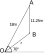
\includegraphics[width=0.3\textwidth]{ex_p_1.pdf}
\end{figure}

To this must be added a displacement of magnitude 

\begin{equation*}
\frac{1}{2}\cdot 10 \cdot 1.5m^2
\end{equation*}

that is $11.25 m$, vertically downwards, represented by the arrow AB.

The sum of these is the displacement OB.

So after 1.5 seconds the ball is at B.

\vspace{1cm}
\hrule
\vspace{1cm}

\begin{minipage}{\textwidth}
Soluzione dell'esercizio \ref{ex_p_2} a pagina \pageref{ex_p_2}\label{sol_p_2}

\begin{figure}[H]
\centering

\includegraphics[width=0.8\textwidth]{ex_p_2.pdf}
\end{figure}

These diagrams were produced by superimposing several diagrams like
those in exercise \ref{ex_p_1}, but at intervals of $0.5s$ that is for

\begin{equation*}
t=0.5,1,1.5,\ldots,n
\end{equation*}


The displacements $\vec{u}t$ in these times have magnitudes $9 m$, $18 m$, $\ldots$.

The vertical displacements have magnitudes $1.25 m$, $5 m$, $11.25 m$, $\ldots$

The points corresponding to $A$ and $B$ at time $t$ are denoted by $At$ and $Bt$.

You can now show the paths by drawing smooth curves through the points $O$,
$B_{0.5}, B_{1}, \ldots$
for the two initial velocities.

\end{minipage}
\vspace{1cm}
\hrule
\vspace{1cm}

Soluzione dell'esercizio \ref{ex_p_3} a pagina \pageref{ex_p_3}\label{sol_p_3}


It is simplest to take the origin at ground level, rather than at the point
from which the ball is served, so add 2 to the $y$-coordinate given by the
general formula. 

If the initial speed of the ball is $p\frac{m}{s}$,


\begin{equation*}
x = pt \textrm{ and }y = 2 - 5t^2
\end{equation*}

Both conditions involve both the $x$- and $y$-coordinates, and the time $t$ is
used as the link.

The ball passes over the net when $12 = pt$, that is $t=\frac{12}{p}$

The value of $y$ is then

\begin{equation*}
2-5\left(
\frac{12}{p}
\right)=2-\frac{720}{p^2}
\end{equation*}

and this must be more than $0.9$, so 

\begin{equation*}
2-\frac{720}{p^2} > 0.9
\end{equation*}

This gives

\begin{equation*}
\frac{720}{p^2} <1.1
\end{equation*}


\begin{equation*}
p>\sqrt{\frac{720}{1.1}}\approx25.6
\end{equation*}

Considering the second constraint: the ball lands when $y = 0$, that is when 
$2 - 5t^2 = 0$, or 


\begin{equation*}
t=\sqrt{\frac{2}{5}}
\end{equation*}

It has then gone a horizontal distance of $p\sqrt{\frac{2}{5}}$
metres, and to satisfy the second condition you need $p\sqrt{\frac{2}{5}} < 18$.

This gives 



\begin{equation*}
p<18\sqrt{\frac{5}{2}}\approx 28.5
\end{equation*}


So the ball can be hit with any speed between about $25.6 \frac{m}{s}$
and
$28.5\frac{m}{s}$

\vspace{1cm}
\hrule
\vspace{1cm}

Soluzione dell'esercizio \ref{ex_p_4} a pagina \pageref{ex_p_4}\label{sol_p_4}

Known variables:

\begin{itemize}
\item[$s$] = $1.25m$
\item[$a$] = $9.81\frac{m}{s}$
\item[$u$] = 0
\item[$t$] = ?
\end{itemize}

The equations linking those variables are:


\setcounter{equation}{0}
\begin{equation}
s=ut+\frac{1}{2}at^2
\end{equation}

\begin{equation*}
s=\frac{1}{2}gt^2
\end{equation*}



\begin{equation*}
t=\sqrt{\frac{2s}{g}}
\end{equation*}


\begin{equation*}
t=\sqrt{
\frac{
2\cdot 1.25
}{
9.81
}
}=0.5s
\end{equation*}

Now consider the horizontal motion.

\begin{itemize}
\item[$s$] = $10m$
\item[$a$] = $0$
\item[$t$] = 0.5s
\item[$u$] = ?
\end{itemize}



\begin{equation*}
\textrm{velocity}
=\frac{
\textrm{displacement}
}{
\textrm{time}
}
\end{equation*}



\begin{equation*}
v=\frac{10}{0.5}=20\frac{m}{s}
\end{equation*}



\vspace{1cm}
\hrule
\vspace{1cm}


Soluzione dell'esercizio \ref{ex_p_5} a pagina \pageref{ex_p_5}\label{sol_p_5}

La risposta corretta è la ``A".

In entrambi i casi i corpi sono soggetti alla forza peso, che è conservativa. 
Durante la caduta l’energia potenziale della forza peso $mgh$ si trasforma in energia cinetica
\begin{equation*}
 \frac{1}{2} mv^2
\end{equation*}

Ne segue che la velocità finale, al termine del percorso, sarà pari a 

\begin{equation*}
v = 2 gh
\end{equation*}
identica per entrambi i corpi.


È evidente che il risultato è indipendente dalla massa del corpo (risposta D)
come pure dall’angolo d’inclinazione del piano (risposta E).
I tempi di caduta sono differenti: quello lungo il piano inclinato dipende dall’angolo
d’inclinazione ed aumenta al diminuire di quest’ultimo.



\vspace{1cm}
\hrule
\vspace{1cm}


